\chapter{雪盖土壤热力过程}
%\addcontentsline{toc}{chapter}{雪盖土壤热力过程}

%\begin{雪盖土壤热力过程}

在雪盖和土壤中,热力过程主要根据热传导第二定律进行描述。假设雪盖土壤无水平物质能量交换,则其垂直方向上的一维能量平衡方程如下:
\begin{equation}\label{eq:1d_energy_balance}
c \frac{\partial T}{\partial t}=-\frac{\partial F}{\partial z}
\end{equation}
其中$c$表示雪盖或土壤的体积热容量(J/m3/K),$T$表示雪盖土壤温度(K),$t$表示时间(s),$z$表示雪盖高度或土壤深度(m),
F表示垂直方向的热传导通量,方向向上为正($\rm W/m^2$),表达式为$F=-\lambda\frac{\partial T}{\partial z}$,$\lambda$表示热力传导率(W/m/K)。
将方程(\ref{eq:1d_energy_balance})进行离散,并结合上边界由大气输送到雪盖土壤表面的热通量$h_s$以及下边界土壤底层的零热通量,
即可求出雪盖土壤的温度扩线,之后再根据相态变化条件对温度进行进一步调整。
\section{温度求解的数值格式}\label{温度求解的数值格式}
在离散上述能量平衡方程时,土壤被划分为10层。每一层土壤的中心深度$z_i$(m)定义为:
\begin{equation}
z_{i}=f_{s} \exp [0.5(i-0.5)]-1
\end{equation}
%
其中尺度因子$f_s=0.025$。这里采用指数定义可以保证土壤接近表面时得到更细的分层,因为土壤水梯度在接近表面时非常大。基于此定义,每一层土壤的厚度$\Delta z_i$(m)可计算为:
\begin{equation}
\Delta z_{i}=\left\{\begin{array}{ll}0.5\left(z_{1}+z_{2}\right) & i=1 \\ 0.5\left(z_{i+1}-z_{i-1}\right) & i=2 \ldots 9 \\ z_{10}-z_{9} & i=10\end{array}\right.
\end{equation}
相邻两层土壤交界处的深度$z_{h,i}$(m)可计算为:
\begin{equation}
z_{h, i}=\left\{\begin{array}{ll}0.5\left(z_{i}+z_{i+1}\right) & i=1 \ldots 9 \\ z_{10}+0.5 \Delta z_{10} & i=10\end{array}\right.
\end{equation}


雪盖位于土壤之上,可根据其厚度划分为至多5层。为与土壤层编号一致,
这里与土壤表层相邻的雪层记为第0层,逐渐向上依次记为第-1层直至至多为第-4层。
记$snl$为划分的雪层总层数的相反数,则最上层雪层即为第$snl+1$层。雪层划分方案如下:\\
当$z_{sno}<0.01$时,$snl=0$,这时积雪较少,不单独划分为层;\\
当$0.01\le z_{sno}\le0.03$时,\\
\begin{equation}
\left\{\begin{array}{c}s n l=-1 \\ \Delta z_{0}=z_{sno}\end{array}\right.
\end{equation}
当$0.03<z_{sno}\le0.04$时,
\begin{equation}
\left\{\begin{array}{c}s n l=-2 \\ \Delta z_{-1}=z_{sno} / 2 \\ \Delta z_{0}=\Delta z_{-1}\end{array}\right.
\end{equation}
当$0.04<z_{sno}\le0.07$时,
\begin{equation}
\left\{\begin{array}{c}s n l=-2 \\ \Delta z_{-1}=0.02 \\ \Delta z_{0}=z_{sno}-\Delta z_{-1}\end{array}\right.
\end{equation}
当$0.12<z_{sno}\le0.18$时,
\begin{equation}
\left\{\begin{array}{c}s n l=-3 \\ \Delta z_{-2}=0.02 \\ \Delta z_{-1}=0.05 \\ \Delta z_{0}=z_{sno}-\Delta z_{-2}-\Delta z_{-1}\end{array}\right.
\end{equation}
当$0.18<z_{sno}\le0.29$时,
\begin{equation}
\left\{\begin{array}{c}s n l=-4 \\ \Delta z_{-3}=0.02 \\ \Delta z_{-2}=0.05 \\ \Delta z_{-1}=\left(z_{sno}-\Delta z_{-3}-\Delta z_{-2}\right) / 2 \\ \Delta z_{0}=\Delta z_{-1}\end{array}\right.
\end{equation}
当$0.29<z_{sno}\le0.41$时,
\begin{equation}
\left\{\begin{array}{c}s n l=-4 \\ \Delta z_{-3}=0.02 \\ \Delta z_{-2}=0.05 \\ \Delta z_{-1}=0.11 \\ \Delta z_{0}=z_{sno}-\Delta z_{-2}-\Delta z_{-1}\end{array}\right.
\end{equation}
当$0.41<z_{sno}\le0.64$时,
\begin{equation}
\left\{\begin{array}{c}s n l=-5 \\ \Delta z_{-4}=0.02 \\ \Delta z_{-3}=0.05 \\ \Delta z_{-2}=0.11 \\ \Delta z_{-1}=\left(z_{sno}-\Delta z_{-3}-\Delta z_{-2}\right) / 2 \\ \Delta z_{0}=\Delta z_{-1}\end{array}\right.
\end{equation}
当$z_{sno}>0.64$时,
\begin{equation}
\left\{\begin{array}{c}s n l=-5 \\ \Delta z_{-4}=0.02 \\ \Delta z_{-3}=0.05 \\ \Delta z_{-2}=0.11 \\ \Delta z_{-1}=0.23 \\ \Delta z_{0}=z_{sno}-\Delta z_{-3}-\Delta z_{-2}-\Delta z_{-1}\end{array}\right.
\end{equation}
$z_{h,0}=0$为雪盖底层与土壤表层交界处的高度。将此交界面以上的高度定义为负值,则每一层雪的中心高度$z_i$(m)与相邻两层雪交界处的高度$z_{h,i}$(m)计算为:
\begin{equation}
\begin{array}{l}z_{i}=z_{h, i}-0.5 \Delta z_{i} \quad i=0, \ldots, s n l+1 \\ z_{h, i}=z_{h, i+1}-\Delta z_{i+1} \quad i=-1, \ldots, s n l\end{array}
\end{equation}
注意,在计算雪盖土壤温度之前,若有降雪发生($p_i>0$)且无雪盖分层($snl=0$),则此时需通过下式判断第一层雪能否形成:
\begin{equation}
\begin{array}{c}z_{sno}=z_{sno}+\frac{p_{i} \Delta t}{\rho_{\text {sno,new }}} \\ W_{sno}=W_{sno}+p_{i} \Delta t\end{array}
\end{equation}
其中$\rho_{sno,new}$表示新降的干雪密度($\rm kg/m^3$),计算方案为 \citet{anderson1976point}:
\begin{equation}
\rho_{sno, new}=\begin{cases}
169 & \text { 当 } T_{atm}>T_{f}+2.0 \\ 
50+1.7\left(T_{atm}-T_{f}+15\right)^{1.5}  & \text { 当 } T_{f}-15.0<T_{atm} \leq T_{f}+2.0 \\ 
50 & \text { 当 } T_{atm} \leq T_{f}-15.0
\end{cases}
\end{equation}
若此时$z_{sno} \geq 0.01$,则按如上方式对积雪进行分层,且每一层雪的温度取为$T_p$,液态水含量取为0,固态水含量按雪层厚度权重分配$W_{sno}$。若之前已有雪层且此时有降雪发生,则第一层雪的相关物理量作如下更新:
\begin{equation}
w_{ice, snl+1}=w_{ice, snl+1}+p_{i} \Delta t
\end{equation}
\begin{equation}
\Delta z_{snl+1}=\Delta z_{snl+1}+\frac{p_{i} \Delta t}{\rho_{sno, new}}
\end{equation}
\begin{equation}
z_{snl+1}=z_{h, snl+1}-0.5 \Delta z_{snl+1}
\end{equation}
\begin{equation}
z_{h, snl}=z_{h, snl+1}-\Delta z_{snl+1}
\end{equation}
雪盖土壤垂直分层及其热传导过程示意图见图 \ref{fig:雪盖土壤垂直分层及其热传导过程示意图}。其中土壤热力学状态变量
(如雪盖土壤温度$T_i$,热力传导率$\lambda_i$,体积比热容$c_i$等)定义在每一层的中间深度,从第$i+1$层到第$ i $层的热传导通量$F_i$定义在两层的交界处,它可离散为:
\begin{equation}
F_{i}=\lambda\left[z_{h, i}\right] \frac{T_{i}-T_{i+1}}{z_{i}-z_{i+1}}
\end{equation}
其中$\lambda\left[z_{h,i}\right]$表示第$i+1$层与第 $i$ 层交界处的热力传导率。求解$\lambda\left[z_{h,i}\right]$时,
假设从第$i+1$层到第$ i $层的热传导通量等于从第$i+1$层到第$i+1$层与第$i$层交界层的热传导通量,又等于从交接层到第$i$层的热传导通量,即
\begin{equation}
\lambda\left[z_{h, i}\right] \frac{T_{i}-T_{i+1}}{z_{i}-z_{i+1}}=\lambda_{i+1} \frac{T_{m}-T_{i+1}}{z_{h, i}-z_{i+1}}=\lambda_{i} \frac{T_{i}-T_{m}}{z_{i}-z_{h, i}}
\end{equation}
即可通过后两项解出第$i+1$层与第$i$层交界处的温度$T_m$;再将$T_m$代回,通过前两项即可解出$\lambda\left[z_{h,i}\right]$为:
\begin{equation}
\lambda\left[z_{h, i}\right]=\begin{cases}
\frac{\lambda_{i} \lambda_{i+1}\left(z_{i}-z_{i+1}\right)}{\lambda_{i}\left(z_{h, i}-z_{i+1}\right)+\lambda_{i+1}\left(z_{i}-z_{h, i}\right)} & i=snl+1, \ldots, 9 \\ 
0 & i=10
\end{cases}
\end{equation}
特殊地,对于土壤与雪盖的交界面,为防止最下层雪盖厚度过大导致$\lambda\left[z_{h,i}\right]$计算不准,
当$i=0$且$\left(z_{i+1}-z_{h,i}\right)<\left(z_{h,i}-z_i\right)$时,$\lambda\left[z_{h,i}\right]$重新计算为:
\begin{equation}
\lambda\left[z_{h,i}\right]=\frac{2 \lambda_{i} \lambda_{i+1}}{\lambda_{i}+\lambda_{i+1}} \geq 0.5 \lambda_{i+1}
\end{equation}
{
\begin{figure}[]
\centering
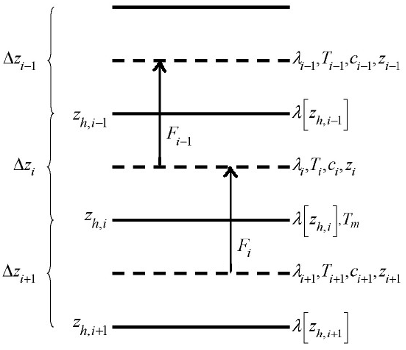
\includegraphics{Figures/雪盖土壤热力过程/雪盖土壤垂直分层及其热传导过程示意图.png}
\caption{雪盖土壤垂直分层及其热传导过程示意图。}
\label{fig:雪盖土壤垂直分层及其热传导过程示意图}
\end{figure}
}


基于以上离散方案,第$ i $层雪盖土壤的能量平衡方程可表达为:
\begin{equation}
\frac{c_{i} \Delta z_{i}}{\Delta t}\left(T_{i}^{n+1}-T_{i}^{n}\right)=F_{i}-F_{i-1}
\end{equation}

其中$\Delta t$表示积分时间步长,$n$表示积分步数。此方程采用Crank-Nicholson半隐式格式求解,既包含前一时刻已有的温度与热通量信息,又包含后一时刻的预报信息。于是此方程可写为如下形式:
\begin{equation}
\frac{c_{i} \Delta z_{i}}{\Delta t}\left(T_{i}^{n+1}-T_{i}^{n}\right)=\alpha\left(F_{i}^{n}-F_{i-1}^{n}\right)+(1-\alpha)\left(F_{i}^{n+1}-F_{i-1}^{n+1}\right)
\end{equation}
其中权重因子$\alpha=0.5$。此方程展开,即有
\begin{equation}
\begin{aligned} \frac{c_{i} \Delta z_{i}}{\Delta t}\left(T_{i}^{n+1}-T_{i}^{n}\right)=& 0.5\left\{\lambda\left[z_{h, i}\right] \frac{T_{i}^{n}-T_{i+1}^{n}}{z_{i}-z_{i+1}}-\lambda\left[z_{h, i-1}\right] \frac{T_{i-1}^{n}-T_{i}^{n}}{z_{i-1}-z_{i}}\right.\\ &\left.+\lambda\left[z_{h, i}\right] \frac{T_{i}^{n+1}-T_{i+1}^{n+1}}{z_{i}-z_{i+1}}-\lambda\left[z_{h, i-1}\right] \frac{T_{i-1}^{n+1}-T_{i}^{n+1}}{z_{i-1}-z_{i}}\right\} \end{aligned}
\end{equation}
将所有层雪盖土壤能量平衡方程联立,可形成关于预报变量$T_{i-1}^{n+1},T_i^{n+1}$和$T_{i+1}^{n+1}$的三对角方程组形式:$r_i=a_iT_{i-1}^{n+1}+b_iT_i^{n+1}+c_iT_{i+1}^{n+1}$,
其中$a_i$,$b_i$,$c_i$分别为三对角矩阵中上三角、对角线和下三角位置中的元素。用追赶法解此方程组即可快速求得每一层雪盖土壤的温度$T_i^{n+1}$。


对于雪盖土壤的中间层($snl+1<i<10$),三对角矩阵中的系数表达如下:
\begin{equation}
\begin{array}{c}a_{i}=-(1-\alpha) \frac{\Delta t}{c_{i} \Delta z_{i}} \frac{\lambda\left[z_{h, i-1}\right]}{z_{i}-z_{i-1}} \\ b_{i}=1+(1-\alpha) \frac{\Delta t}{c_{i} \Delta z_{i}}\left[\frac{\lambda\left[z_{h, i-1}\right]}{z_{i}-z_{i-1}}+\frac{\lambda\left[z_{h, i}\right]}{z_{i+1}-z_{i}}\right] \\ c_{i}=-(1-\alpha) \frac{\Delta t}{c_{i} \Delta z_{i}} \frac{\lambda\left[z_{h, i}\right]}{z_{i+1}-z_{i}} \\ r_{i}=T_{i}^{n}+\alpha \frac{\Delta t}{c_{i} \Delta z_{i}} \lambda\left[z_{h, i}\right] \frac{T_{i}^{n}-T_{i+1}^{n}}{z_{i}-z_{i+1}}-\lambda\left[z_{h, i-1}\right] \frac{T_{i-1}^{n}-T_{i}^{n}}{z_{i-1}-z_{i}}\end{array}
\end{equation}
对于雪盖土壤的顶层和底层,需要考虑对应的边界条件:\\
(1) 对于雪盖土壤顶层($i=snl+1$),来自大气的热通量$h_s$将会进入到地表中,即
\begin{equation}
h_{s}^{n+1}=-\alpha F_{i-1}^{n}-(1-\alpha) F_{i-1}^{n+1}
\end{equation}
对$h_s^{n+1}$采用一阶泰勒展开近似,则顶层能量平衡方程变为:
\begin{equation}
\begin{array}{l}\frac{c_{i} \Delta z_{i}}{\Delta t}\left(T_{i}^{n+1}-T_{i}^{n}\right)=h_{s}^{n+1}+\alpha F_{i}^{n}+(1-\alpha) F_{i}^{n+1} \\ \approx h_{s}^{n}+\frac{\partial h_{s}}{\partial T_{i}}\left(T_{i}^{n+1}-T_{i}^{n}\right)+\alpha \lambda\left[z_{h, i}\right] \frac{T_{i}^{n}-T_{i+1}^{n}}{z_{i}-z_{i+1}}+(1-\alpha) \lambda\left[z_{h, i}\right] \frac{T_{i}^{n+1}-T_{i+1}^{n+1}}{z_{i}-z_{i+1}}\end{array}
\end{equation}
于是,基于此方程可得雪盖土壤顶层的三对角矩阵系数为:
\begin{equation}
\begin{array}{c}a_{i}=0 \\ b_{i}=1+\frac{\Delta t}{c_{i} \Delta z_{i}}\left[(1-\alpha) \frac{\lambda\left[z_{h, i}\right]}{z_{i+1}-z_{i}}-\frac{\partial h_{s}}{\partial T_{i}}\right] \\ c_{i}=-(1-\alpha) \frac{\Delta t}{c_{i} \Delta z_{i}} \frac{\lambda\left[z_{h, i}\right]}{z_{i+1}-z_{i}} \\ r_{i}=T_{i}^{n}+\frac{\Delta t}{c_{i} \Delta z_{i}}\left[h_{s}^{n}-\frac{\partial h_{s}}{\partial T_{i}} T_{i}^{n}+\alpha \lambda\left[z_{h, i}\right] \frac{T_{i}^{n}-T_{i+1}^{n}}{z_{i}-z_{i+1}}\right]\end{array}
\end{equation}
这里进入到地表的热通量$h_s$($\rm W/m^2$)具体表达为:
\begin{equation}
\begin{array}{c}h_{s}=S_{g}+L_{g}\left(T_{g}\right)-H_{g}\left(T_{g}\right)-\lambda E_{g}\left(T_{g}\right)+H_{p r c g}\left(T_{g}\right) \\ \frac{\partial h_{s}}{\partial T_{i}}=\frac{\partial L_{g}}{\partial T_{i}}-\frac{\partial H_{g}}{\partial T_{i}}-\frac{\partial \lambda E_{g}}{\partial T_{i}}+\frac{\partial H_{p r c g}}{\partial T_{i}}\end{array}
\end{equation}
其中$S_g$和$L_g$分别表示地表吸收的净太阳辐射和净长波辐射($\rm W/m^2$)。$h_s$中的各个能量组份已在前面各节有所介绍,这里对于$L_g$的计算给予补充:
\begin{equation}
L_{g}=L_{p g} \downarrow+\varepsilon_{g} L_{b g} \downarrow-L_{g} \uparrow
\end{equation}
其中$L_{pg}\downarrow$表示植被覆盖下地表吸收的下行长波辐射(见章节 \ref{长波净辐射通量}),$L_{bg}\downarrow$表示无植被覆盖下到达地表的下行长波辐射:
\begin{equation}
L_{b g} \downarrow=\left(1-f_{ sig }\right) L \downarrow
\end{equation}
$L_g\uparrow$表示地表发出的上行长波辐射:
\begin{equation}
L_{g} \uparrow=\varepsilon_{g} \sigma T_{g}^{4}
\end{equation}
另外,对于潜热通量系数$\lambda$,当雪盖土壤顶层不存在液态水时,$\lambda$取为升华潜热系数$\lambda_s$,即:
\begin{equation}
\lambda=\left\{\begin{array}{lr}\lambda_{s} & \text { 当 } w_{liq, s n l+1}=0 \text { 并且 } w_{ice, s n l+1}>0 \\ \lambda_{v} & \text { 其他情况 }\end{array}\right.
\end{equation}
其中$w_{liq,snl+1}$和$w_{ice,snl+1}$分别表示雪盖土壤顶层的液态水和固态水含量 ($\rm kg/m^2$,其计算见章节~\ref{sec:土壤水的运动})。

在模式中,地表温度$T_g$与$T_{snl+1}$取为同一值,但$T_{snl+1}$表示第一层雪盖或土壤的平均温度,与实际的$T_g$相比具有减弱的日变化幅度。
为改进这一缺陷,在求解第一层能量平衡方程时,其厚度$\Delta z_i$作以下调整,以求得更接近实际的$T_g$:
\begin{equation}
\Delta z_{i}=0.5\left[z_{i}-z_{h, i-1}+c_{a}\left(z_{i+1}-z_{h, i-1}\right)\right]
\end{equation}
其中调整参数$c_a=0.34$。\\
(2) 对于土壤底层($i=10$),假设热传导通量为0,则能量平衡方程变为:
\begin{equation}
\frac{c_{i} \Delta z_{i}}{\Delta t}\left(T_{i}^{n+1}-T_{i}^{n}\right)=-\alpha \lambda\left[z_{h, i-1}\right] \frac{T_{i-1}^{n}-T_{i}^{n}}{z_{i-1}-z_{i}}-(1-\alpha) \lambda\left[z_{h, i-1}\right] \frac{T_{i-1}^{n+1}-T_{i}^{n+1}}{z_{i-1}-z_{i}}
\end{equation}
于是,基于此方程可得土壤底层的三对角矩阵系数为:
\begin{equation}
\begin{array}{c}a_{i}=-(1-\alpha) \frac{\Delta t}{c_{i} \Delta z_{i}} \frac{\lambda\left[z_{h, i-1}\right]}{z_{i}-z_{i-1}} \\ b_{i}=1+(1-\alpha) \frac{\Delta t}{c_{i} \Delta z_{i}} \frac{\lambda\left[z_{h, i-1}\right]}{z_{i}-z_{i-1}} \\ c_{i}=0 \\ r_{i}=T_{i}^{n}-\alpha \frac{\Delta t \lambda\left[z_{h, i-1}\right]}{c_{i} \Delta z_{i}} \frac{T_{i-1}^{n}-T_{i}^{n}}{z_{i-1}-z_{i}}\end{array}
\end{equation}


下面给出各层雪盖土壤的热力传导率$\lambda_i$与体积热容量$c_i$的计算方案:\\

根据\citet{farouki1981thermal},土壤热力传导率$\lambda_i$ (W/m/K, $i=1,..,10$)的计算公式如下:

\begin{equation}
\lambda_{i}=\left\{\begin{array}{ll}K_{e, i} \lambda_{sat, i}+\left(1-K_{e, i}\right) \lambda_{d r y, i} & S_{r, i}>1 \times 10^{-7} \\ \lambda_{d r y, i} & S_{r, i} \leq 1 \times10^{-7}\end{array}\right.
\end{equation}
其中,$\lambda_{sat,i}$与$\lambda_{dry,i}$分别是饱和土壤和干土壤的热力传导率,由地表参数数据集提供,$S_{r,i}$表示土壤相对于其饱和状态的潮湿程度:
\begin{equation}
S_{r, i}=\left(\frac{w_{liq, i}}{\rho_{liq} \Delta z_{i}}+\frac{w_{ice, i}}{\rho_{ice} \Delta z_{i}}\right) \frac{1}{\theta_{sat, i}} \leq 1
\end{equation}
$K_{e,i}$表示Kersten数,它是$S_{r,i}$的函数:
\begin{equation}
K_{e, i}=\left\{\begin{array}{ll}\log _{10} S_{r, i}+1 \geq 0 & \text{ 当 } T_{i} \geq T_{f} \text{ 时 } \\ S_{r, i} & \text{ 当 } T_{i}<T_{f} \text{ 时 }\end{array}\right.
\end{equation}
当$T_i<T_f$时,饱和土壤热力传导率$\lambda_{sat,i}$需根据已有$\lambda_{sat,i}$结合水和冰的热力传导率$\lambda_{liq}$,$\lambda_{ice}$进行调整:
\begin{equation}
\lambda_{\text {sat}, i}=\lambda_{\text {sat}, i}\left(\frac{\lambda_{\text {ice}}}{\lambda_{\text {liq}}}\right)^{\theta_{\text {sat}, i}\left(1-\frac{w_{liq, i}}{w_{liq}, i+w_{ice, i}}\right)}
\end{equation}
$\theta_{sat,i}$表示第$ i $层土壤的孔隙度。


根据 \citet{jordan1991one},雪盖热力传导率$\lambda_i$ (W/m/K, $i=snl+1,..,0$)的计算公式如下:
\begin{equation}
\lambda_{i}=\lambda_{a}+\left(7.75 \times 10^{-5} \rho_{sno, i}+1.105 \times 10^{-6} \rho_{sno, i}^{2}\right)\left(\lambda_{ice}-\lambda_{a}\right)
\end{equation}
其中$\lambda_a$表示空气的热力传导率(W/m/K),$\rho_{sno,i}$表示第 $i$ 层雪的平均密度($\rm kg/m^3$):
\begin{equation}
\rho_{sno, i}=\frac{w_{liq, i}+w_{ice, i}}{\Delta z_{i}}
\end{equation}



根据 \citet{de1963thermal},土壤体积热容量$c_i$(J/m3/K, $i=1,..,10$)的计算公式如下:
\begin{equation}
c_{i}=c_{s, i}\left(1-\theta_{sat, i}\right)+\frac{w_{ice, i}}{\Delta z_{i}} C_{pi}+\frac{w_{liq, i}}{\Delta z_{i}} C_{p l}
\end{equation}
其中$c_{s,i}$表示干土壤的体积热容量,由地表参数数据集提供。若地表有积雪但无雪层,则积雪的热容量也需考虑:
\begin{equation}
c_{i}=c_{s,i}\left(1-\theta_{sat, i}\right)+\frac{w_{ice, i}}{\Delta z_{i}} C_{pi}+\frac{w_{liq,i}}{\Delta z_{i}} C_{pl}+\frac{W_{sno}}{\Delta z_{i}} C_{pi}
\end{equation}
对于雪盖体积热容量$c_i$ (J/m3/K, $i=snl+1,..,0$),其计算公式为:
\begin{equation}
c_{i}=\frac{w_{ice, i}}{\Delta z_{i}} C_{pi}+\frac{w_{liq, i}}{\Delta z_{i}} C_{pl}
\end{equation}


\section{温度的相态变化调整}
通过解能量平衡方程组计算出下一时刻的雪盖土壤温度后,需要考虑相态变化过程对温度进行调整。在模式中,相态变化发生的条件为:\\
若$T_i^{n+1}>T_f$并且$w_{ice,i}>0$ \ \   \ \  \ \   固态水融化\\
若$T_i^{n+1}<T_f$并且$w_{liq,i}>0$  \ \   \ \  \ \         液态水冻结\\
一个特殊情况是,当土壤表面积雪存在$\left(W_{sno}>0\right)$但并无雪层$\left(snl=0,z_{sno}<0.01\right)$时,\\
若$T_1^{n+1}>T_f$      \ \   \ \  \ \                 积雪融化\\
以上三种情况下,$T_i^{n+1}$被调整为$T_f$。


相态变化的程度是由$T_i^{n+1}$调整为$T_f$后产生的能量冗余或亏损决定的。温度调整后,能量的冗余或亏损$H_i$($\rm W/m^2$)计算如下:
\begin{equation}
H_{i}=\left\{\begin{array}{lr}h_{s}^{n}+\frac{\partial h_{s}}{\partial T_{i}}\left(T_{f}-T_{i}^{n}\right)+\alpha F_{i}^{n}+(1-\alpha) F_{i}^{n+1}-\frac{c_{i} \Delta z_{i}}{\Delta t}\left(T_{f}-T_{i}^{n}\right) & i=s n l+1 \\ \alpha\left(F_{i}^{n}-F_{i-1}^{n}\right)+(1-\alpha)\left(F_{i}^{n+1}-F_{i-1}^{n+1}\right)-\frac{c_{i} \Delta z_{i}}{\Delta t}\left(T_{f}-T_{i}^{n}\right) & s n l+1<i<10 \\ -\alpha F_{i-1}^{n}-(1-\alpha) F_{i-1}^{n+1}-\frac{c_{i} \Delta z_{i}}{\Delta t}\left(T_{f}-T_{i}^{n}\right) & i=10\end{array}\right.
\end{equation}
对应地,相态变化的质量调整量为$H_{m}=\frac{H_{i} \Delta t}{L_{f}}$,其中$L_f$表示固态水液化潜热(J/kg)。当固态水融化条件被满足且$H_m>0$时,固态水含量被调整为:
\begin{equation}
w_{ice, i}^{n+1}=w_{ice, i}^{n}-H_{m} \geq 0
\end{equation}
当液态水冻结条件被满足且$H_m<0$时,固态水含量被调整为:
\begin{equation}
w_{ice, i}^{n+1}=\min \left(w_{ice, i}^{n}-H_{m}, w_{liq, i}^{n}+w_{ice, i}^{n}\right)
\end{equation}
以上情况液态水含量均被调整为:
\begin{equation}
w_{liq, i}^{n+1}=w_{liq, i}^{n}+w_{ice, i}^{n}-w_{ice, i}^{n+1} \geq 0
\end{equation}
若水分调节过程不足以消耗全部的能量冗余或填补全部的能量亏损,
则在相态变化过程之后再次进行能量结余计算:$ H_{i *}=H_{i}+\frac{L_{f}\left(w_{ice, i}^{n+1}-w_{ice, i}^{n}\right)}{\Delta t}$。
若$\left|H_{i\ast}\right|>0$,则此部分能量可用来再次暖化或冷却雪盖土壤层,温度调整如下:
\begin{equation}
T_{i}^{n+1}=\left\{\begin{array}{lr}T_{f}+\frac{\Delta t}{c_{i} \Delta z_{i}} H_{i *} /\left(1-\frac{\Delta t}{c_{i} \Delta z_{i}} \frac{\partial T_{s}}{\partial T_{i}}\right) & i=s n l+1 \\ T_{f}+\frac{\Delta t}{c_{i} \Delta z_{i}} H_{i *} & i \neq s n l+1 \\ T_{f} & w_{liq, i}^{n+1} * w_{ice, i}^{n+1}>0\end{array}\right.
\end{equation}
对于特殊的土壤表面积雪融化的情形,当$H_m>0$时,雪水当量减少为
\begin{equation}
W_{sno}^{n+1}=W_{s no}^{n}-H_{m} \geq 0
\end{equation}
同样,雪的厚度减少为
\begin{equation}
z_{sno}^{n+1}=\frac{W_{sno}^{n+1}}{W_{sno}^{n}} z_{sno}^{n}
\end{equation}
若积雪融化不足以消耗全部的能量冗余,则剩余能量$H_{1\ast}$为
\begin{equation}
H_{1 *}=H_{1}+\frac{L_{f}\left(W_{sno}^{n+1}-W_{sno}^{n}\right)}{\Delta t}
\end{equation}
此时$H_{1\ast}$将作为新的$H_1$对第一层土壤进行上述相态变化计算。


综上,若发生土壤表面积雪融化的情形,则用于相态变化的能量累计$E$为:
\begin{equation}
E=\frac{L_{f}\left(W_{sno}^{n}-W_{sno}^{n+1}\right)}{\Delta t}+\sum_{i=1}^{10} \frac{L_{f}\left(w_{ice, i}^{n}-w_{ice, i}^{n+1}\right)}{\Delta t}
\end{equation}
否则,
\begin{equation}
E=\sum_{i=1}^{s n l+1} \frac{L_{f}\left(w_{ice, i}^{n}-w_{ice, i}^{n+1}\right)}{\Delta t}
\end{equation}
以上过程即是雪盖土壤温度计算的全部过程。得到$T_i^{n+1}$后,地表发出的上行长波辐射$L_g\uparrow$,感热通量$H_g$与潜热通量$\lambda E_g$需再做一次更新以作为输出的状态变量,
其中用于蒸发的水汽不能超过雪盖土壤顶层的总含水量$\left(w_{liq,snl+1}^{n+1}+w_{ice,snl+1}^{n+1}\right)/\Delta t$,
否则地表蒸发水汽取为$\left(w_{liq,snl+1}^{n+1}+w_{ice,snl+1}^{n+1}\right)/\Delta t$,产生的能量误差将加到感热通量上。
